% !TEX root = ../../Dissertation.tex

\begin{refsection}

\chapter[Vanadium Trigermanium \ch{VG\lowercase{e}3}]{Geometric and Electronic Structures of \ch{VGe3^{-/0}}} \label{VGe3}


\definecolor{shadecolor}{gray}{0.85}
\begin{shaded}
\textbf{This chapter is based on the paper:}\\
Pham, L. N.; Nguyen, M. T. Insights into Geometric and Electronic Structures of \ch{VGe3^{-/0}} Clusters from Anion Photoelectron Spectrum Assignment. \textit{J. Phys. Chem. A} \textbf{2017}, 121, 6949–6956.  \textit{Reprinted with permission from Journal of Chemical Theory and Computation. Copyright 2017. American Chemical Society.} \textcolor{blue}{The \href{https://pubs.acs.org/doi/suppl/10.1021/acs.jpca.7b07459/suppl_file/jp7b07459_si_001.pdf}{Supporting Information} is available online}.

\emph{My contribution to this work was theoretical calculations, data analysis, discussion, writing of the first draft and revision.}
\newpage
\end{shaded}


\section{Introduction}

Germanium is one of the potential candidates for high-performance electronic transistors. \cite{c5:1} With a search for new materials based on germanium, several types of pure and metal-doped clusters of germanium have been theoretically studied and experimentally synthesized. \cite{c5:2, c5:3, c5:4, c5:5, c5:6, c5:7, c5:8, c5:9, c5:10, c5:11, c5:12} Usually, germanium clusters are doped with transition metals, and the obtained clusters can be detected and characterized by, among others, anion photoelectron (\acrshort{pe}) spectroscopy. In principle, mass-selected anionic clusters irradiated with high-energy beams of photons are ionized, and signals of removed electrons are then recorded in anion \acrshort{pe} spectra. Dozens of germanium clusters doped with metals such as Sc, V, Ti, Co, Ru, Nb, and Au have been studied by this method. \cite{c5:2, c5:6, c5:7, c5:8, c5:9, c5:11} 





Typically, experimentalists can identify with anion \acrshort{pe} spectroscopy in conjunction with mass spectroscopy the sizes and ionization energies of clusters. For clusters containing transition metals, electronic structures and insights of their excited states are usually quite complicated. As can be seen from previous reports \cite{c5:13, c5:14, c5:15} on pure germanium clusters and our recent study on digermanium doped with titanium, \cite{c5:16} energy degeneracy of states significantly affects the anion \acrshort{pe} spectra. In such cases, more than one electronic transition can cause one visible band in the spectrum. Thus, although the measured anion \acrshort{pe} spectrum seems to be simple to understand, elucidation of the electronic transitions underlying it is not straightforward. In light of the reports mentioned, it is reasonable to expect that energetically degenerate states exist in other doped germanium clusters and are involved in the generation of anion \acrshort{pe} spectra.





Of the germanium clusters doped with metals, vanadium trigermanium is one of the simplest clusters spectroscopically characterized using the \acrshort{pe} technique. \cite{c5:6} For the sake of comprehension, Figure \ref{fig5:spectrum} reproduces the experimental spectrum reported in ref \citenum{c5:6}. Accordingly, five distinguishable bands are recorded corresponding to five ionizations of the anion \ch{VGe3-}. First, the lowest vertical ionization is located at 2.02 eV whose adiabatic ionization energy is 1.73 eV. At higher levels, inner electrons are photodetached, and thereby four more \acrshort{pe} bands are obtained. One of the latter bands has an ionization energy of 2.80 eV, and three remaining ones are >3.0 eV (3.13, 3.40, and 3.60 eV). On the basis of ionization energy and density functional theory (\acrshort{dft}) calculations, the most stable isomers of both anionic and neutral \ch{VGe3^{–/0}} were claimed to have a rhombic form (Figure \ref{fig5:VGe3-iso}a). A quintet state ($^5$A) and a quartet one ($^4$A) are determined to be the ground states of the anionic and neutral clusters, respectively. \cite{c5:6} A recent \acrshort{dft} study using the B3LYP functional \cite{c5:17} pointed out that the most stable isomers of \ch{VGe3^{–/0}} are both in the tetrahedral shape (Figure \ref{fig5:VGe3-iso}c). While a quartet state ($^4$A) is the neutral global minimum, a singlet state (C$_{3v}$, $^1$A$_1$) is the anionic ground state.







\begin{figure}[htb!]
	\centering
	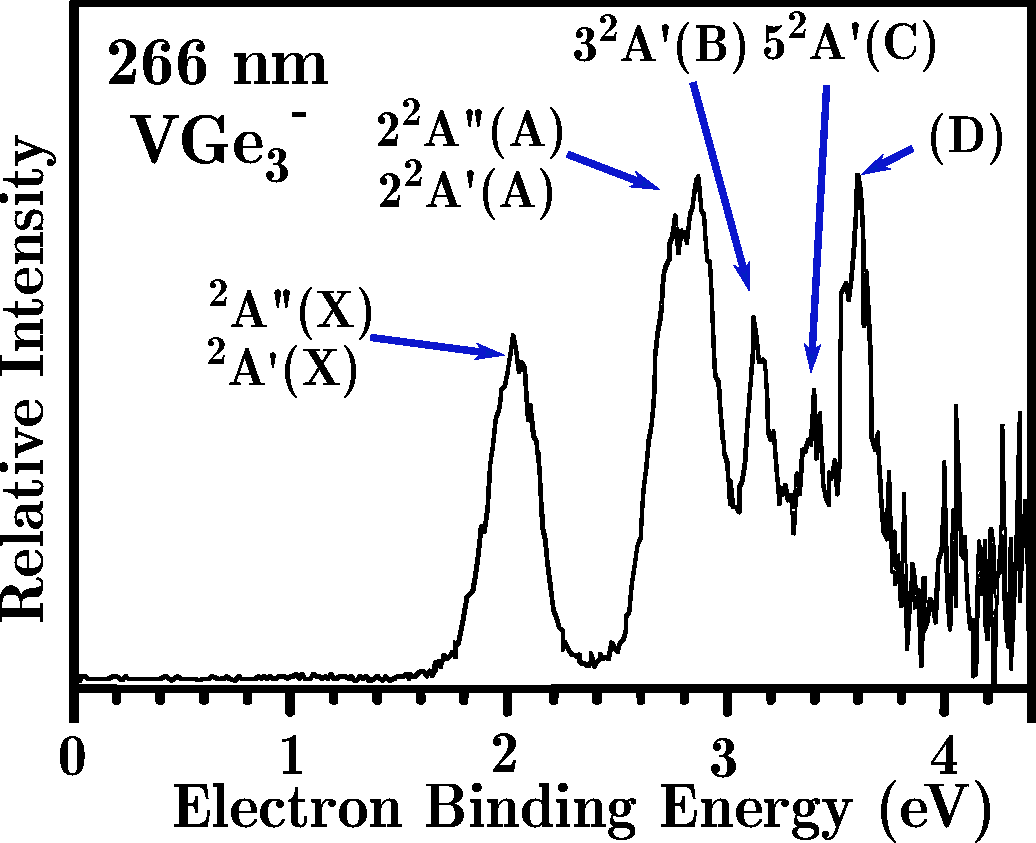
\includegraphics[width=0.4\textwidth]{VGe3-spectrum}
	\caption{Anion photoelectron spectrum of \ch{VGe3-} with five distinguishable bands denoted as X, A, B, C, and D is taken from ref \citenum{c5:6}. Reproduced with permission from ref \citenum{c5:6}. Copyright 2015 American Chemical Society.} 
	\label{fig5:spectrum}
\end{figure} 






\begin{figure}[htb!]
	\centering
	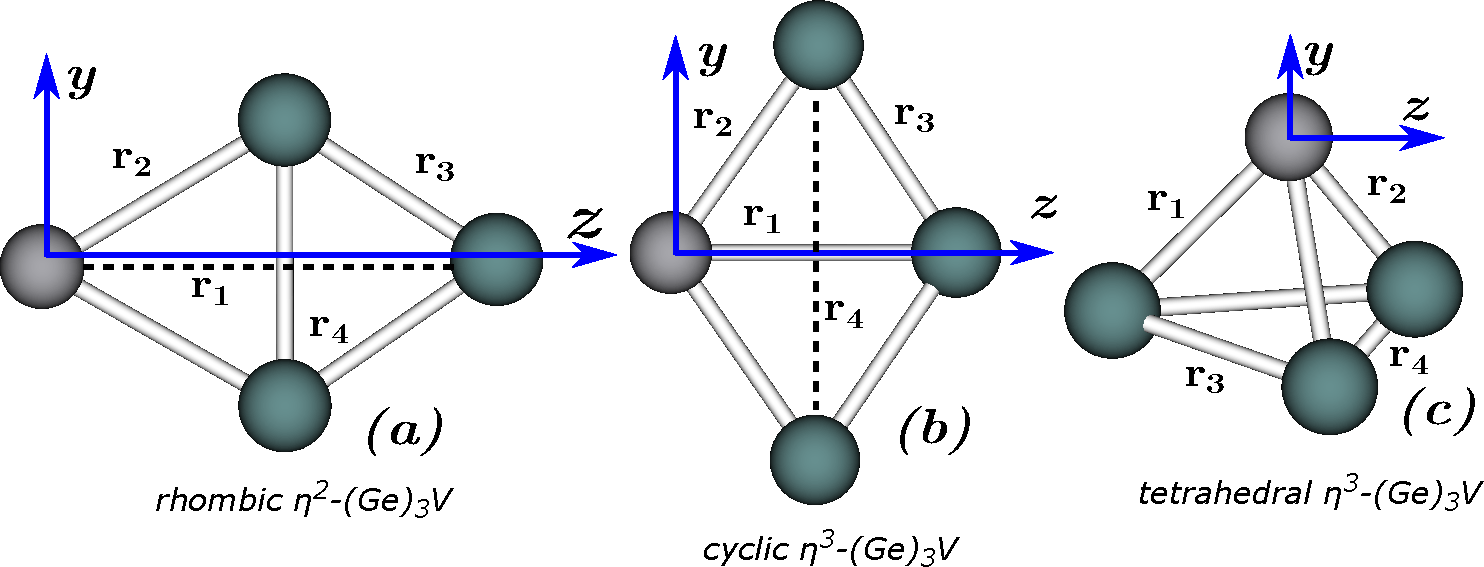
\includegraphics[width=0.75\textwidth]{VGe3-isomers}
	\caption{Three possible geometries of \ch{VGe3^{–/0}} and the coordinate systems employed.} 
	\label{fig5:VGe3-iso}
\end{figure} 




Beside the confusing notations of electronic states assigned in the two previous reports, \cite{c5:6, c5:17} one can recognize a disagreement on the identity of the most stable isomers and their ground states. Furthermore, the conclusions on the ground states given in the latter report are doubtful, as they simply violate the spin selection rule. In fact, starting from a singlet state, one cannot obtain a quartet state upon ionization. Apart from such doubtful conclusions, our pre-evaluations also reveal that the rhombic isomer is not the most stable geometry of \ch{VGe3^{–/0}} as reported in a previous report. \cite{c5:6} More importantly, other excited experimental bands appearing in the spectrum of the anion \ch{VGe3-} still need to be fully understood. In this context, we set out to reinvestigate the geometric and electronic structures of both anionic and neutral clusters \ch{VGe3^{–/0}} making use of several reliable methods of quantum chemical theory.




\section{Computational Details}


Geometrical structures of \ch{VGe3^{–/0}} clusters are optimized using the multireference \acrshort{casscf}/\acrshort{caspt2} \cite{c5:18} method. In this method, the correlation energy is expected to be well-recovered, and therefore, the global minima of both the anion and neutral can definitely be identified from relative energies. From previous reports \cite{c5:6, c5:17} and our preliminary evaluations (data given in Figure \href{https://pubs.acs.org/doi/suppl/10.1021/acs.jpca.7b07459/suppl_file/jp7b07459_si_001.pdf}{\textcolor{blue}{S1}} of the \href{https://pubs.acs.org/doi/suppl/10.1021/acs.jpca.7b07459/suppl_file/jp7b07459_si_001.pdf}{\textcolor{blue}{Supporting Information}}), three low-lying isomers of \ch{VGe3^{–/0}} (Figure \ref{fig5:VGe3-iso}) are more stable than the others, and hence, these isomers are considered in this optimization step. The coordinate systems used in our calculations are displayed in Figure \ref{fig5:VGe3-iso}.




For \acrshort{caspt2} calculations, all five 3d and one 4s orbitals of vanadium are included in the active space of \acrshort{casscf} wave functions. We should note that 4s orbitals of three germanium atoms are likely involved in photodetachment processes which appear as the highest band in the spectrum of \ch{VGe3-}. Nonetheless, inclusion of all 4s orbitals in the active space would make the \acrshort{casscf}/\acrshort{caspt2} calculations practically prohibited. As a consequence, only nine 4p orbitals of three germanium atoms are taken into account. As vanadium has 5 valence electrons and three germanium atoms have 6 4p valence ones, complete configuration state functions (\acrshort{csf}s) are generated on the basis of \acrshort{casscf}(11,15) and \acrshort{casscf}(12,15) wave functions including 11 (for the neutral) and 12 (for the anion) electrons distributed in 15 active orbitals, respectively. Since the relative energies obtained are of paramount importance in determination of the global minima, and moreover the optimal geometrical structures are going to be used in all extra single-point calculations afterward, subsequent \acrshort{caspt2} optimization is implemented in conjunction with relatively large basis sets. The \acrshort{ano}-RCC basis set with contraction of [7s6p4d3f2g] \cite{c5:19} and of [6s5p3d1f] \cite{c5:20} is used for vanadium and germanium, respectively. All geometry optimizations are conducted with the MOLCAS 8.0 code. \cite{c5:21} All 3p and inner-core electrons of both vanadium and germanium are kept frozen in the recovery of dynamic correlation under treatment of second-order perturbation.





To confirm the results obtained above, several additional single-point electronic energies are computed making use of \acrshort{caspt2} optimal geometries. For the purpose of ground-state identification, the coupled-cluster theory \acrshort{rccsd}(T) is an obvious choice. For finding of appropriate \acrshort{dft} functionals to treat a system like \ch{VGe3^{–/0}}, the pure exchange-correlation generalized gradient approximation (\acrshort{gga}) functional BP86 \cite{c5:22, c5:23} is selected because it performs better than other tested functionals (refer to Table \href{https://pubs.acs.org/doi/suppl/10.1021/acs.jpca.7b07459/suppl_file/jp7b07459_si_001.pdf}{\textcolor{blue}{S1}} for more details). All computations using these two single-reference methods are done with regard to the electronic structure of each state emerged from \acrshort{casscf} wave functions. In addition to single-reference methods (\acrshort{dft} and \acrshort{rccsd}(T)), single-point multireference configuration interaction (\acrshort{mrci}) energies of a few accessible states are also calculated to further support the assignment. The Davidson correction for the quadruple contributions is used to improve \acrshort{mrci} energies as well. For a balance between accuracy and our computing resources, the relatively large basis set (quadruple-$\zeta$ aug-cc-pVQZ-DK \cite{c5:24, c5:25}) is employed for both vanadium and germanium atoms. All \acrshort{rccsd}(T) calculations utilize the same electron-correlation schemes used in previous \acrshort{caspt2} calculations. In \acrshort{mrci}(Q) calculations, due to technical shortcomings we cannot include 15 3d orbitals of three germanium atoms, and they are not correlated in \acrshort{mrci}(Q) calculations. Only 4s and 4p orbitals of Ge atoms are thus included. In the internally contracted \acrshort{mrci}(Q) calculations, all \acrshort{csf}s with coefficients larger than or equal to 0.05 generated from prior \acrshort{casscf} calculations are taken into account.




On the basis of optimal geometries of the ground and low-lying states obtained from \acrshort{caspt2} optimizations, vertical (\acrshort{vde}s) and adiabatic (\acrshort{ade}s) detachment energies can be drawn. \acrshort{vde}s are calculated by making use of the initial state (usually the anionic ground state). \acrshort{rccsd}(T) and \acrshort{mrci}(Q) single-point energies are computed using the program MOLPRO 2012. \cite{c5:26} We should stress that, for small clusters, \acrshort{zpe} corrections are not important as proved elsewhere; \cite{c5:27} this is because \acrshort{zpe}s of all isomers considered are small and nearly the same. Hence all relative energies are derived from pure electronic energies without \acrshort{zpe} corrections. Corrections of scalar relativistic effects are taken into consideration using the second-order Douglas–Kroll–Hess Hamiltonian of all electrons. \cite{c5:28}



Symmetry plays a vital role in most calculations in this work. As seen in Figure \ref{fig5:VGe3-iso}a,b, the rhombic or cyclic symmetry is simple. Our pre-evaluation shows that both isomers exhibit a C$_{2v}$ spatial symmetry. For the tetrahedral isomer (Figure \ref{fig5:VGe3-iso}c) \ch{VGe3^{–/0}} can be in a C$_{3v}$ form (indeed \ch{VGe3-} is). However, spatial symmetrical wave functions of this point group (non-Abelian) cannot be treated in the currently used program packages. Therefore, we use the lower-symmetry C$_s$ point group. All symmetrical operations for these three isomers can be deduced from Figure \ref{fig5:VGe3-iso}.




Finally, Franck–Condon factors of electronic transitions which contribute to the first band in the anion \acrshort{pe} spectrum of \ch{VGe3-} are simulated as a further confirmation of our assignment. The first band can be simulated because only harmonic frequencies of the involved states underlying this band can be accessed. To obtain equilibrium geometrical parameters and analytic vibrational frequencies of involved states, geometries of considered states are optimized using the BP86 functional in conjunction with the basis set def2-TZVP \cite{c5:29} as implemented in the TURBOMOLE 7.1 package, \cite{c5:30} and harmonic vibrational frequencies are calculated analytically at the same level. We choose the BP86 pure exchange-correlation \acrshort{gga} functional because this functional reproduces quite well experimental detachment energies of \ch{VGe3^-} as presented later in this work. All parameters are provided as input for simulations up to 10 quanta, which are done with the aid of the MolFC code. \cite{c5:31} 




\section{Results and Discussion}

\subsection{The Most Stable Isomer and Ground States}


The most stable isomers of \ch{VGe3^{-/0}} are identified on the basis of relative energies obtained after geometry optimizations. Optimized \acrshort{caspt2} bond lengths of the three low-lying isomers of \ch{VGe3^{-/0}} and \acrshort{caspt2} relative energies of several low-lying states are given in Table \ref{tbl5:RE}. Relative energies calculated using the BP86 functional and \acrshort{rccsd}(T) are also provided in this table. Unequivocally, the $^1$A' state (with respect to C$_s$ symmetry, but C$_{3v}$ point group being the true spatial symmetry of this state) of the tetrahedral isomer is positioned at the lowest point on the potential surface of \ch{VGe3-}. At the \acrshort{caspt2} level, the second-lowest states of the anion are the two nearly degenerate $^3$A' and $^3$A" states of the tetrahedral $\eta^{3}$-\ch{(Ge3)V-}. Both triplet states are $\sim$0.6 eV higher in energy than the $^1$A'. The most stable cyclic anion (Figure \ref{fig5:VGe3-iso}b) is the $^3$B$_2$, which is energetically higher than the ground state $^1$A' by $\sim$0.7 eV, whereas the high-spin $^5$B$_2$ state is determined to be $\sim$1.0 eV less stable.




\begin{table}[htb!]
    \centering
    \begin{threeparttable}
    \caption{Determination of the Ground States at BP86, \acrshort{rccsd}(T), and \acrshort{caspt2} Levels\tnote{(a)}}
    \label{tbl5:RE}
    \begin{tabular}{@{}lcccccc@{}}
    \toprule
    \multicolumn{1}{c}{\multirow{2}{*}{isomer}} & \multirow{2}{*}{state} & \multirow{2}{*}{sym} & \multirow{2}{*}{\begin{tabular}[c]{@{}c@{}}\acrshort{caspt2} geometry (\AA) \\ r$_1$, r$_2$, r$_3$, r$_4$\end{tabular}} & \multicolumn{3}{c}{relative energy (eV)} \\ \cmidrule(l){5-7} 
    \multicolumn{1}{c}{}           &       &       &          & BP86   & \acrshort{rccsd}(T) & \acrshort{caspt2}      \\ \midrule
\begin{tabular}[c]{@{}l@{}}tetrahedral \\ $\eta^3$-(\ch{Ge3)V-} \end{tabular}  & $^1$A'      & C$_s$      & 2.35, 2.35, 2.70, 2,70   & 0.00   & 0.00     & 0.00        \\
                                   & $^1$A"      & C$_s$      & 2.37, 2.44, 2.70, 2.52   &        &          & 0.89        \\
                                   & $^3$A'      & C$_s$      & 2.46, 2.39, 2.60, 2.83   & 0.40   & 0.83     & 0.60        \\
                                   & $^3$A"      & C$_s$      & 2.37, 2.44, 2.75, 2.52   & 0.39   & 0.82     & 0.60        \\
                                   & $^5$A'      & C$_s$      & 2.53, 2.48, 2.58, 2.71   & 0.80   & 1.29     & 1.21        \\
                                   & $^5$A"      & C$_s$      & 2.55, 2.53, 2.56, 2.56   & 0.84   & 1.27     & 1.07        \\
\begin{tabular}[c]{@{}l@{}}rhombic \\ $\eta^2$-(\ch{Ge3)V-} \end{tabular}      & $^5$B$_2$   & C$_{2v}$   & 4.34, 2.63, 2.42, 2.57   & 0.41   & 0.62     & 1.01        \\
                                   & $^5$A$_2$   & C$_{2v}$   & 4.40, 2.69, 2.42, 2.60   & 0.84   & 0.83     & 1.28        \\
\begin{tabular}[c]{@{}l@{}}cyclic  \\ $\eta^3$-(\ch{Ge3)V-} \end{tabular}       & $^1$A$_1$   & C$_{2v}$   & 2.74, 2.39, 2.42, 3.95   & 0.87   & 0.48     & 0.80        \\
                                   & $^3$B$_2$   & C$_{2v}$   & 2.63, 2.37, 2.47, 4.07   & 0.52   & 0.87     & 0.68        \\
                                   & $^3$A$_2$   & C$_{2v}$   & 2.72, 2.39, 2.47, 4.03   & 0.89   & 1.23     & 1.09        \\
                                   & $^5$A$_1$   & C$_{2v}$   & 2.90, 2.43, 2.44, 3.91   & 1.67   & 1.07     & 0.88        \\
                                   & $^5$B$_1$   & C$_{2v}$   & 3.25, 2.45, 2.43, 3.64   & 0.76   & 1.18     & 0.89        \\
                                   & $^5$B$_2$   & C$_{2v}$   & 2.64, 2.45, 2.41, 4.09   & 0.89   & 1.29     & 1.02        \\
\begin{tabular}[c]{@{}l@{}}tetrahedral \\ $\eta^3$-(\ch{Ge3})V \end{tabular}   & $^2$A'      & C$_s$      & 2.42, 2.36, 2.59, 2.79   & 1.88   & 1.89     & 1.70        \\
                                   & $^2$A"      & C$_s$      & 2.34, 2.40, 2.72, 2.53   & 1.89   & 1.88     & 1.69        \\
                                   & $^4$A'      & C$_s$      & 2.46, 2.44, 2.60, 2.72   & 2.40   & 2.84     & 2.39        \\
                                   & $^4$A"      & C$_s$      & 2.47, 2.47, 2.61, 2.61   & 2.13   & 2.56     & 2.15        \\
                                   & $^6$A'      & C$_s$      & 2.80, 2.57, 2.41, 3.29   & 2.88   & 3.26     & 2.96        \\
                                   & $^6$A"      & C$_s$      & 2.50, 2.63, 2.57, 2.64   & 3.00   & 3.36     & 3.00        \\
\begin{tabular}[c]{@{}l@{}}rhombic \\ $\eta^2$-(\ch{Ge3})V \end{tabular}   & $^4$B$_2$   & C$_{2v}$   & 4.21, 2.47, 2.44, 2.52   & 2.39   & 2.55     & 2.25        \\
                                   & $^4$A$_2$   & C$_{2v}$   & 4.15, 2.52, 2.42, 2.69   & 2.37   & 2.46     & 2.29        \\
\begin{tabular}[c]{@{}l@{}}cyclic \\  $\eta^3$-(\ch{Ge3})V \end{tabular}  & $^2$B$_2$   & C$_{2v}$   & 2.55, 2.36, 2.50, 4.12   & 2.86   & 2.84     & 2.70        \\
                                   & $^4$B$_1$   & C$_{2v}$   & 2.84, 2.42, 2.44, 3.95   & 2.54   & 3.03     & 2.50        \\
                                   & $^4$B$_2$   & C$_{2v}$   & 2.51, 2.46, 2.41, 4.17   & 2.61   & 3.05     & 2.56        \\
                                   & $^6$A$_1$   & C$_{2v}$   & 2.64, 2.53, 2.38, 4.13   & 2.57   & 3.01     & 2.59        \\ \bottomrule
    \end{tabular}
    \begin{tablenotes}
        \item[(a)] \acrshort{rccsd}(T) and BP86 energies are obtained using \acrshort{caspt2}-optimized geometries. The true symmetrical point group for the anion is C$_{3v}$, but C$_s$ is used. All values are calculated from total electronic energies without \acrshort{zpe}.
    \end{tablenotes}
    \end{threeparttable}
    \end{table}





As for the neutral ground state, two states $^2$A' and $^2$A" have the lowest relative energies and are nearly degenerate. Relative energies of $^2$A' and $^2$A" states with respect to the anionic ground state $^1$A' are 1.70 and 1.69 eV, respectively. Their degeneracy is reconfirmed with relative energies calculated at the BP86 and \acrshort{rccsd}(T) levels as seen in Table \ref{tbl5:RE}. In this case, the \acrshort{caspt2} method reproduces excellently the experimental \acrshort{ade} of the first band, being 1.70 versus 1.73 eV. This agreement between the calculated and experimental ionization energy strongly reinforces our conclusion on the global minima of \ch{VGe3^{-/0}}.




The remaining low-lying states of the neutral including those of the rhombic and cyclic isomers are all significantly higher than both degenerate states $^2$A' and $^2$A". Finally, as an extra confirmation, all values of relative energies calculated at the BP86 and \acrshort{rccsd}(T) levels support \acrshort{caspt2} results that the $^1$A' state of the tetrahedral $\eta^3$-\ch{(Ge3)V-} is the ground state of the anion \ch{VGe3-} ($^1$A$_1$ for the anion under C$_{3v}$) and the neutral has two competitive doublet states for its ground state. 




All the results above can give us a clear conclusion that the tetrahedral geometry of both anion and neutral are the most stable isomers. Under the cooled experimental condition, the tetrahedral structures of \ch{VGe3^{-/0}} are likely to be much more populated in comparison to the others. This result disagrees with the conclusion reported elsewhere \cite{c5:6} that the rhombic form is the most stable one of \ch{VGe3^{-/0}}. The more recent \acrshort{dft} computations \cite{c5:17} using the B3LYP functional somewhat agree with our results in terms of the stable geometrical structures, and the ground state of the anionic \ch{VGe3-} ($^1$A'), but not for the neutral ground state. Note that the neutral ground state has a C$_s$ symmetry (determined by our calculations) instead of a C$_{3v}$ as reported in ref \citenum{c5:17}. Geometrical structure is changed from C$_{3v}$ to C$_s$ upon ionization. Such a change will be analyzed in the next section.





\subsection{Electronic Structures and One-Electron Electronic Transitions}



As proven above, the tetrahedral isomer, namely, tetrahedral $\eta^3$-\ch{(Ge3)V^{-/0}}, is the most stable geometrical structure of both anionic and neutral \ch{VGe3^{-/0}}. Using spatial symmetry C$_s$, the anionic ground state is $^1$A', and both doublet $^2$A' and $^2$A" states are nearly degenerate, vying for the competitive ground state of the neutral. Therefore, to predict the electronic transitions that do not violate the selection rule, electronic structures of ground states and other possibly excited ones of the tetrahedral $\eta^3$-\ch{(Ge3)V^{-/0}} need to be understood.




The leading configurations of both anionic and neutral ground states obtained from \acrshort{casscf} wave functions are presented in Table \ref{tbl5:ldconfig}. Some other low-lying states of the tetrahedral $\eta^3$-\ch{(Ge3)V^0} are also given in this table. The occupied pseudonatural orbitals of $^1$A' (C$_s$ tetrahedral $\eta^3$-\ch{(Ge3)V-} are displayed in Figure \ref{fig5:VGe3-orbs}. In general, these active-space orbitals are quite complex in terms of their original components. Indeed, each of them has a contribution from valence atomic orbitals (\acrshort{ao}s) of vanadium and germanium, but the schemes of contributions are expected to be not the same for all orbitals. While the molecular orbitals (\acrshort{mo}s) 34a' and 37a' are remarkably dominated with the trigermanium moiety's 2p orbitals, all the remaining ones are largely contributed by valence \acrshort{ao}s of vanadium (3d and 4s \acrshort{ao}s). A graphic visualization in Figure \ref{fig5:VGe3-orbs} gives more details of the components of these \acrshort{mo}s.

\begin{figure}[htb!]
    \centering
    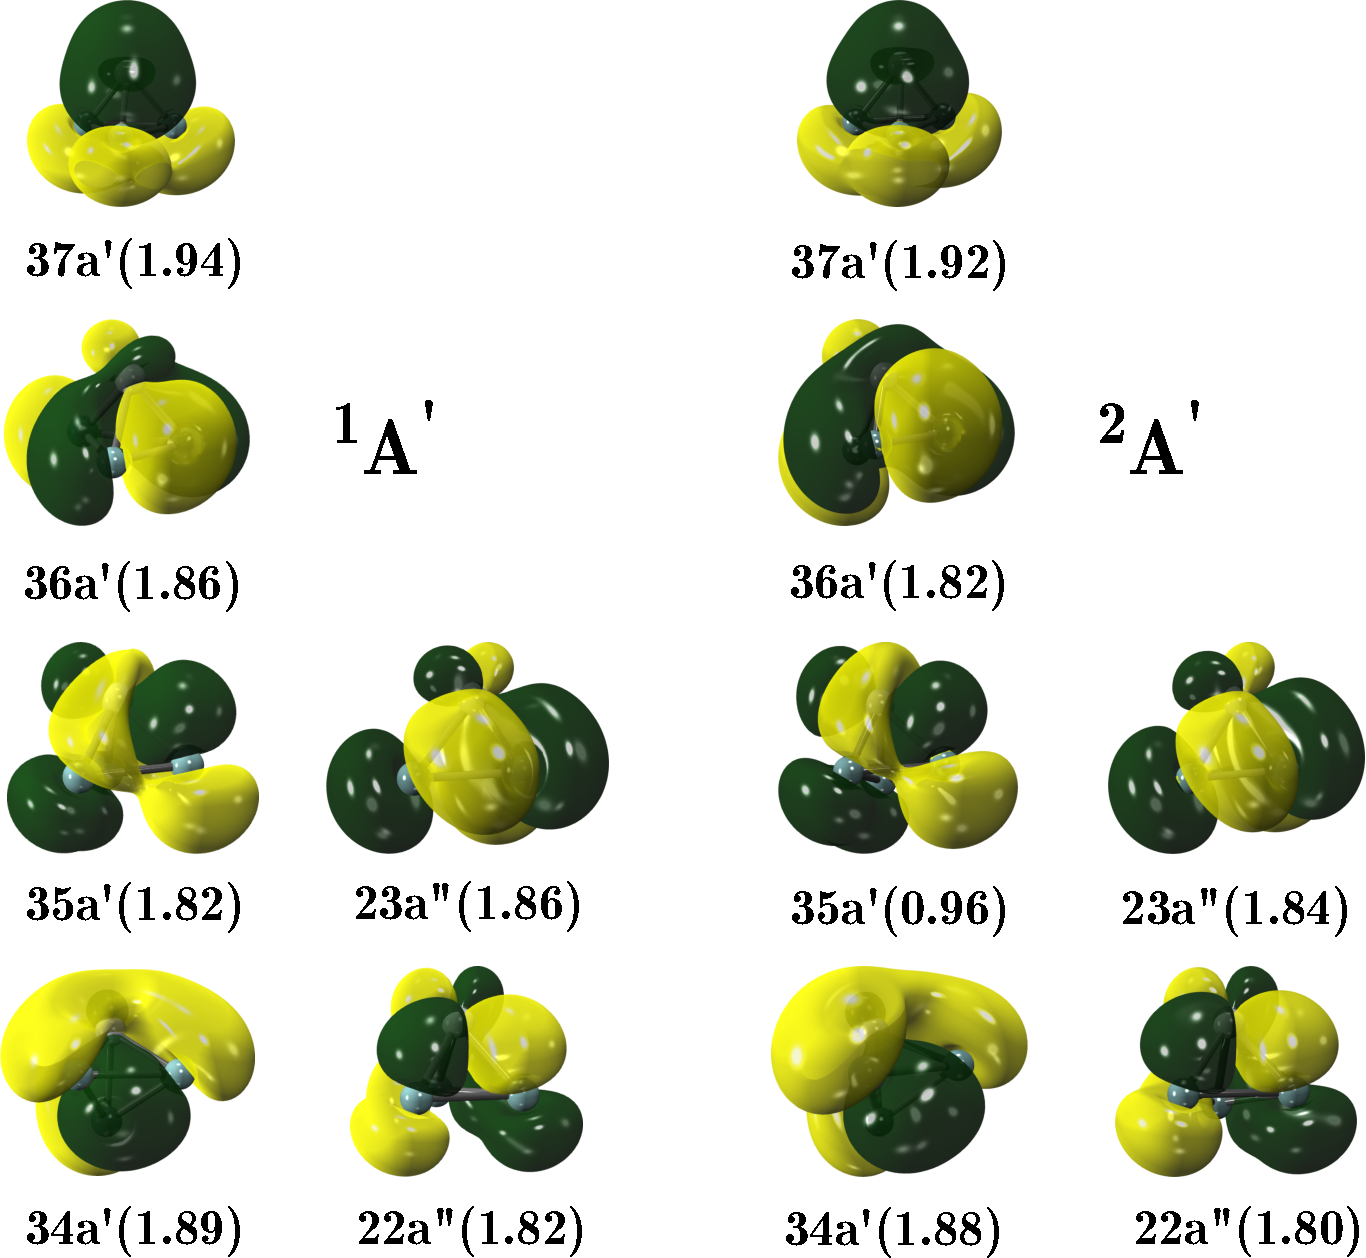
\includegraphics[width=0.55\textwidth]{1A1-2A1-orbitals}
    \caption{Occupied pseudonatural orbitals in the active space of $^1$A' (C$_s$) and corresponding active orbitals of $^2$A'. Orbitals are obtained from \acrshort{casscf} wave functions. The average occupation numbers are given in parentheses. The metal atom V is on the top of the tetrahedral $\eta^3$-\ch{(Ge3)V} isomer.} 
    \label{fig5:VGe3-orbs}
\end{figure} 


Our analyses show that both \acrshort{mo}s 35a' and 22a" mainly have, one by one, contributions from two 3d orbitals of vanadium (3d$_{yz}$, 3d$_{x^2-y^2}$) and (3d$_{xy}$, 3d$_{xz}$). Both \acrshort{mo}s 36a' and 23a" possess stronger components of the metallic orbitals 3d$_{yz}$ and 3d$_{xz}$, respectively. Appearance of the 4s and 3d$_{z^2}$ orbitals of vanadium in occupied orbitals of the anionic ground state is not significant. Figure \ref{fig5:VGe3-orbs} shows the tiny contributions of these two metallic orbitals in the \acrshort{mo}s 34a' and 37a'.


The similarity of features between neutral and anionic ground states can be observed from the visualization in Figure \ref{fig5:VGe3-orbs}. The two \acrshort{mo} sets of $^1$A' and $^2$A' reflect these similar features in each pair of \acrshort{mo}s, except for the occupation number of \acrshort{mo}s 35a' (1.82 versus 0.96). Such a similarity suggests that ionization can occur from the \acrshort{mo} 35a' of the anionic ground state $^1$A' with removal of one electron, and the expected state $^2$A' is formed. This ionization process is noted as $^1$A' $\longrightarrow$ 1$^2$A' in Table \ref{tbl5:ldconfig}, and the ionized orbital can be implicitly withdrawn by comparing two leading configurations of both $^1$A' and $^2$A'. Besides, one can also find major components of the singly occupied orbital noted as [3d$_{yz}$, 3d$_{x^2-y^2}$ + 4p] for this ionization process.


\begin{landscape}
\begin{table}[htb!]
    \centering
    \begin{threeparttable}
    \caption{\acrshort{casscf} Leading Configurations of Anionic and Neutral Ground States, and Electronic Transitions Allowed by Selection Rules}
    \label{tbl5:ldconfig}
    \begin{tabular}{@{}ccccll@{}}
    \toprule
    isomer  & state & leading configuration  & weight (\%) & \multicolumn{1}{c}{ionization} & ionized orbital\tnote{(b)}             \\ \midrule
    \multirow{8}{*}{\begin{tabular}[c]{@{}l@{}}tetrahedral \\ $\eta^3$-\ch{(Ge3)V}\end{tabular}} & $^1$A'   & 34a'$^2$ 35a'$^2$ 36a'$^2$ 37a'$^2$ 38a'$^0$ 22a"$^2$ 23a"$^2$ & 67          &            &                               \\
        & 1$^2$A'  & 34a'$^2$ 35a'$^1$ 36a'$^2$ 37a'$^2$ 38a'$^0$ 22a"$^2$ 23a"$^2$ & 67  & $^1$A' $\longrightarrow$ 1$^2$A' & 35a' {[}3d$_{yz}$, 3d$_{x^2-y^2}$ + 4p{]} \\
        & 2$^2$A'  & 34a'$^2$ 35a'$^2$ 36a'$^1$ 37a'$^2$ 38a'$^0$ 22a"$^2$ 23a"$^2$ & 66  & $^1$A' $\longrightarrow$ 2$^2$A' & 36a' {[}3d$_{yz}$ + 4p{]}          \\
        & 3$^2$A'  & 34a'$^2$ 35a'$^2$ 36a'$^2$ 37a'$^1$ 38a'$^0$ 22a"$^2$ 23a"$^2$ & 46  & $^1$A' $\longrightarrow$ 3$^2$A' & 37a' {[}4s + 4p{]}            \\
        & 4$^2$A'  & 34a'$^2$ 35a'$^2$ 36a'$^0$ 37a'$^1$ 38a'$^2$ 22a"$^2$ 23a"$^2$ & 31  &            &                               \\
        & 5$^2$A'  & 34a'$^1$ 35a'$^2$ 36a'$^2$ 37a'$^2$ 38a'$^0$ 22a"$^2$ 23a"$^2$ & 49  & $^1$A' $\longrightarrow$ 5$^2$A' & 34a' {[}3d$_{z^2}$ + 4p{]}          \\
        & 1$^2$A"  & 34a'$^2$ 35a'$^2$ 36a'$^2$ 37a'$^2$ 38a'$^0$ 22a"$^1$ 23a"$^2$ & 66  & $^1$A' $\longrightarrow$ 1$^2$A" & 22a" {[}3d$_{xy}$, 3d$_{xz}$ + 4p{]}    \\
        & 2$^2$A"  & 34a'$^2$ 35a'$^2$ 36a'$^2$ 37a'$^2$ 38a'$^0$ 22a"$^2$ 23a"$^1$ & 66  & $^1$A' $\longrightarrow$ 2$^2$A" & 23a" {[}3d$_{xz}$ + 4p{]}          \\ \bottomrule  
    \end{tabular}
    \begin{tablenotes}
        \item[(b)] 3d and 4s orbitals originate from vanadium, and 4p orbitals are from three germanium atoms. 4s and 3d$_{z^2}$ \acrshort{ao}s of vanadium have rather minor contributions to two \acrshort{mo}s 37a' and 34a', respectively.
    \end{tablenotes}
    \end{threeparttable}
    \end{table}
\end{landscape}




Most of the bands appearing in the anion \acrshort{pe} spectrum of \ch{VGe3-} are expected to have originated from the anionic ground state. Hence, prediction of possible electronic transitions starting from the anionic ground state can aid us in understanding the bands of the anion \acrshort{pe} spectrum. From the orbital configuration of the $^1$A' state (considered under C$_s$, being $^1$A$_1$ under real C$_{3v}$), one can predict six possible transitions including the transition $^1$A' $\longrightarrow$ 1$^2$A', and six final neutral states can be obtained. Six possible transitions are listed in Table \ref{tbl5:ldconfig} together with corresponding ionized orbitals and their main original \acrshort{ao}s.




With regard to the a' spatial symmetry, apart from the 35a' \acrshort{mo}, three more doubly occupied \acrshort{mo}s (34a', 36a', and 37a'), one by one, can be ionized, and three final states (2$^2$A', 3$^2$A', and 5$^2$A') are theoretically observed. The leading orbital configurations of these three neutral states can be found in Table \ref{tbl5:ldconfig}. Because three ionized \acrshort{mo}s are composed of different \acrshort{ao} components from the vanadium and \ch{Ge3} moiety, ionization energies are expected to be different from each other, and different from the ionization energy of \acrshort{mo} 35a' analyzed above. Particularly, within the a' representation, the orbital 35a' is expected to have the lowest ionization energy, because this orbital is largely contributed to by two valence 3d orbitals of vanadium (3d$_{yz}$ and 3d$_{x^2–y^2}$). The orbital 36a' is underlying the next level of ionization energy, as this \acrshort{mo} has strong 3d$_{yz}$ character. The two remaining \acrshort{mo}s 37a' and 34a' exhibit minor features of the metallic 4s and 3d$_{xy}$ orbitals, respectively, but not the Ge 4p orbitals, and thus need higher photon energies for photodetachments. Taking a closer look at the components of two latter \acrshort{mo}s, we can roughly estimate the ionization energy order. Because the \acrshort{mo} 37a' comprises the vanadium 4s \acrshort{ao}, which is energetically higher than the 3d counterparts, the \acrshort{mo} 37a' is expected to be ionized with a lower energy compared to that of the \acrshort{mo} 34a'.






With respect to the a" spatial orbitals, the \acrshort{mo} 22a" dominantly consists of major metallic features of two 3d \acrshort{ao}s (3d$_{xy}$ and 3d$_{xz}$), and the other one, 23a", has lesser metallic character (3d$_{xz}$) in comparison to that of the \acrshort{mo} 22a". Therefore, we can estimate that ionization energy from the \acrshort{mo} 22a" is lower than that from 23a". As for a comparison, the huge contributions of 3d metallic orbitals to the \acrshort{mo}s 35a' and 22a" are most likely the same, and a similar situation happens for both \acrshort{mo}s 36a' and 23a" with lesser metallic contributions. As a matter of fact, the \acrshort{caspt2}-optimized geometrical structure of the anionic ground state $^1$A' is identified to be in the form of C$_{3v}$ (trigonal pyramid). In this respect, the anionic ground state is the $^1$A$_1$ as mentioned previously. As a result, the two orbitals 35a' and 22a" must be the \acrshort{homo}s of the 2-fold degenerate irreducible representations (irrep) e, and two \acrshort{homo}s - 1 (36a' and 23a") are also degenerate within another 2-fold irrep e. Consequently, one can suggest the leading \acrshort{mo} diagram of the $^1$A' ground state as the one plotted in Figure \ref{fig5:MO-diagram}.



\begin{figure}[htb!]
    \centering
    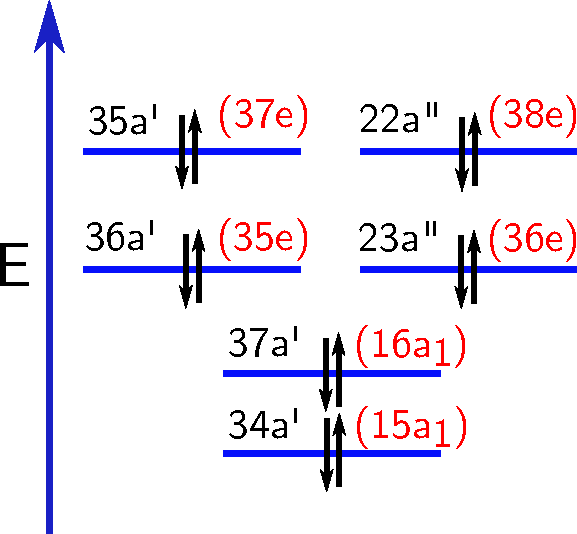
\includegraphics[width=0.35\textwidth]{MO-diagrams}
    \caption{\acrshort{mo} diagram of the anionic ground state $^1$A' ($^1$A$_1$) within the treated active space. Orbital labels with respect to a C$_{3v}$ spatial symmetry are placed in parentheses. The energy ordering is figured out on the basis of the corresponding single-reference wave functions.} 
    \label{fig5:MO-diagram}
\end{figure} 






Turning back to the optimized geometrical structures of tetrahedral $\eta^3$-\ch{(Ge3)V^{-/0}}, we can see that the geometry is distorted upon removal of one electron from the anionic ground state (C$_{3v}$, $^1$A$_1$), giving the neutral ground state ($^2$A' and $^2$A", C$_s$). Such a distortion occurs under a Jahn-Teller effect. This effect does not happen in the anionic ground state $^1$A$_1$, because the two 2-fold degenerate \acrshort{homo}s are doubly occupied, and there is no degeneracy of electronic configurations and no distorted geometry. When one-electron photodetachments take place from one of the degenerate \acrshort{homo}s, two possible electronic configurations of the final state are obtained with the same energy. A Jahn-Teller effect is thus expected to happen inducing a relaxation of the neutral geometry leading to geometry distortion. The distortion directions taking place upon two lowest one-electron ionizations, yielding two distinct $^2$A' and $^2$A" states, are plotted in Figure \ref{fig5:JT}. This is proved in our \acrshort{caspt2} geometry optimization of both $^2$A' and $^2$A" states.




\begin{figure}[htb!]
    \centering
    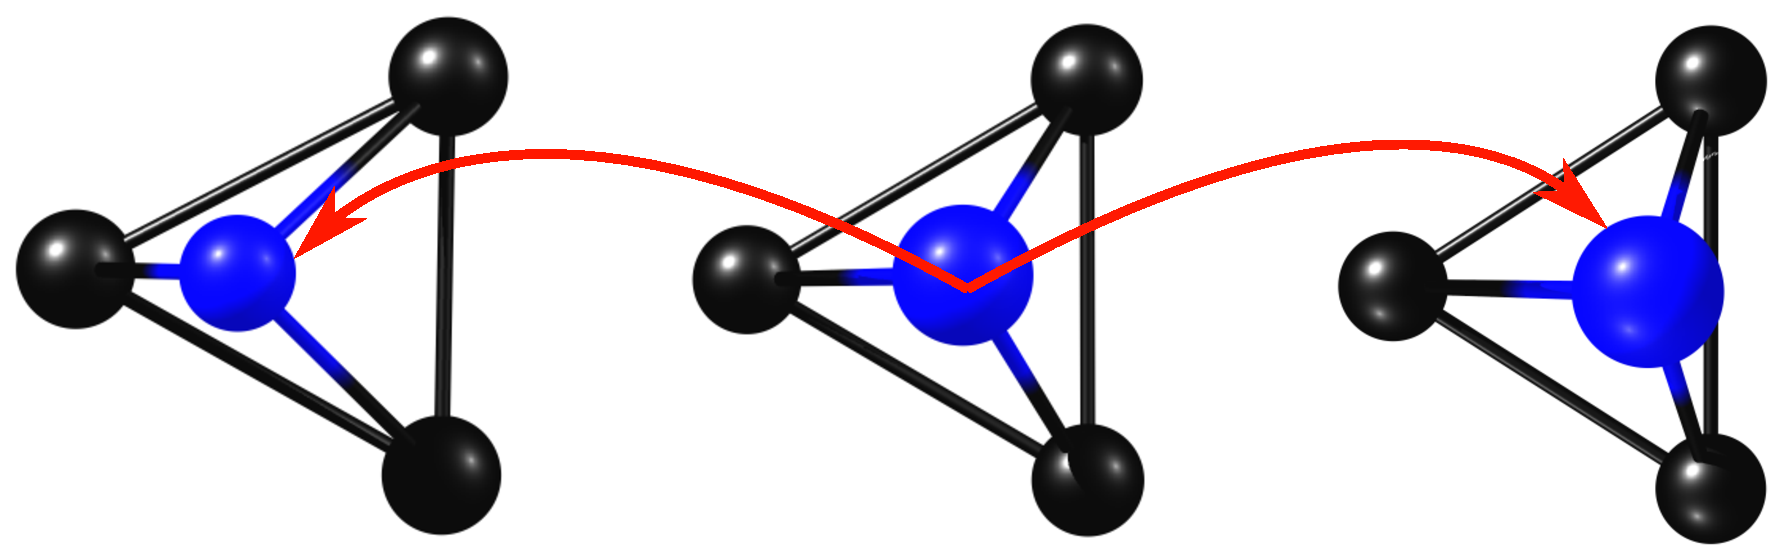
\includegraphics[width=0.5\textwidth]{Jahn-Teller}
    \caption{Two distortion directions under a Jahn–Teller effect upon one-electron photodetachments at the degenerate \acrshort{homo}. The blue atom is vanadium.}
    \label{fig5:JT}
\end{figure} 



\subsection{Anion Photoelectron Spectrum and Band Assignments}


As mentioned above, there are six possible allowed one-electron transitions from the anionic ground state $^1$A' (being $^1$A$_1$). The experimental spectrum points out five distinguished bands of ionization with \acrshort{ade}s ranging from $\sim$2.0 to 3.6 eV, noted as X, A, B, C, and D in Figure \ref{fig5:spectrum}. However, from the electronic structure of the anionic ground state, we know only four levels of ionization energy because the first two levels involve degenerate transitions starting from degenerate orbitals. Thus, the identity of one experimental band cannot be solved. This band is the last one denoted as D with a high detachment energy of 3.60 eV. To assign this band, we need larger active space including all 4s orbitals of three germanium atoms, and the resulting calculations become, at the time being, computationally intractable at the \acrshort{casscf} levels. Therefore, this band will not explicitly be assigned here, but some possible ionization features can be proposed on the basis of an analysis of electronic structure.





To assign bands in the spectrum, we calculate the \acrshort{vde}s of all possible electronic transitions analyzed above using several methods including \acrshort{dft}/BP86, \acrshort{rccsd}(T), \acrshort{mrci}(Q), and \acrshort{caspt2}. These values are provided in Table \ref{tbl5:DE} together with the calculated \acrshort{ade}s of two lowest transitions. The following point has been discussed in a previous section, but for the sake of completeness in spectral assignment, let us state it again.



\begin{table}[htbp!]
    \centering
    \begin{threeparttable}
    \caption{\acrshort{vde}s of Electronic Transitions Originating from the Anionic Ground State $^1$A$_1$}
    \label{tbl5:DE}
    \begin{tabular}{@{}ccccccc@{}}
        \toprule
    \multirow{2}{*}{isomer} & \multirow{2}{*}{state} & \multicolumn{5}{c}{\acrshort{vde} (eV)\tnote{(c)}}                   \\ \cmidrule(l){3-7} 
                                &   & BP86     & \acrshort{rccsd}(T) & \acrshort{mrci}(Q)  & \acrshort{caspt2}  & expt\tnote{(d)}    \\ \midrule
\begin{tabular}[c]{@{}c@{}}tetrahedral \\ $\eta^3$-\ch{(Ge3)V} \end{tabular} & $^1$A'   & 0.00     & 0.00     & 0.00    & 0.00   &          \\
                                    & 1$^2$A'  & 1.93     & 2.02     & 1.87    & 1.78   & 2.02 (X) \\
                                    &          & (1.88)   & (1.89)   & (1.78)  & (1.70) & (1.73)   \\
                                    & 1$^2$A"  & 1.94     & 2.02     & 1.87    & 1.77   &          \\
                                    &          & (1.89)   & (1.88)   & (1.80)  & (1.69) &          \\
                                    & 2$^2$A'  & 2.76     & 2.75     &         & 2.59   & 2.80 (A) \\
                                    & 2$^2$A"  & 2.75     & 2.71     &         & 2.60   &          \\
                                    & 3$^2$A'  & 3.16     &          &         & 2.95   & 3.13 (B) \\
                                    & 4$^2$A'  &          &          &         & 2.98   &          \\
                                    & 5$^2$A'  & 3.53     & 3.38     &         & 3.13   & 3.40 (C) \\ \bottomrule
    \end{tabular}
    \begin{tablenotes}
        \item[(c)] Values are calculated without \acrshort{zpe}; in the parentheses are \acrshort{ade}s. \acrshort{ade}s and \acrshort{vde}s are calculated making use of the \acrshort{caspt2}-optimized geometries of involved states.
        \item[(d)] Experimental values are taken from ref \citenum{c5:6}.
    \end{tablenotes} 
    \end{threeparttable}
    \end{table}





First of all, ionization energies (\acrshort{ade}s and \acrshort{vde}s) again quantitatively confirm the \acrshort{mo} diagram of the $^1$A$_1$ state in Figure \ref{fig5:MO-diagram}. There are clearly two pairs of degenerate \acrshort{mo}s with hierarchical levels of ionization energy. Usually, a ground-ground electronic transition is responsible for the first level of ionization energy, namely, the band X, in \acrshort{pe} spectra. In the present situation, two transitions from the anionic ground state $^1$A$_1$ to two competitive neutral ground states $^2$A' and $^2$A" are responsible for the X band. Because these two electronic transitions, $^1$A$_1$ $\longrightarrow$ 1$^2$A' and $^1$A$_1$ $\longrightarrow$ 1$^2$A", simultaneously start from the same anionic ground state, they should have equal probability to appear in the anion \acrshort{pe} spectrum. As stated above, our calculated \acrshort{ade}s of these two transitions amount to $\sim$1.70 eV at the \acrshort{caspt2} level, which are in excellent agreement with the experimental \acrshort{ade} of 1.73 eV of the X band. The \acrshort{mrci}(Q) also reproduces these \acrshort{ade}s quite well, being 1.78 and 1.80 eV, respectively.





As additional synergism, two single-reference methods give deviations of $\sim$0.16 eV in comparison to experiment. With respect to the \acrshort{vde}, the \acrshort{mrci}(Q) and \acrshort{caspt2} slightly underestimate the experimental \acrshort{vde} (1.87 and 1.78 versus 2.02 eV). Better results are obtained using \acrshort{dft}/BP86 and especially the coupled-cluster theory \acrshort{rccsd}(T). The \acrshort{rccsd}(T) almost recovers the experimental \acrshort{vde} value of 2.02 eV. Again, these results explicitly point toward two transitions $^1$A$_1$ $\longrightarrow$ 1$^2$A' and $^1$A$_1$ $\longrightarrow$ 1$^2$A" being responsible for the X band.





The next level of ionization energy belongs to band A with an experimental \acrshort{vde} of 2.80 eV. From the \acrshort{mo} diagram of $^1$A' (Figure \ref{fig5:MO-diagram}), two ionization processes happening from two degenerate \acrshort{mo}s 36a' and 23a" are expected to underlie this band. Indeed, the \acrshort{caspt2} method predicts two transitions $^1$A$_1$ $\longrightarrow$ 2$^2$A' and $^1$A$_1$ $\longrightarrow$ 2$^2$A" having \acrshort{vde}s of 2.59 and 2.60 eV, respectively. These are in good correlation with experimental data of 2.80 eV. Moreover, with calculated values being $\sim$0.05 eV below experiment, both \acrshort{dft}/BP86 and \acrshort{rccsd}(T) results again reinforce our assignment for this band. Hence, the two states 2$^2$A' and 2$^2$A" are concurrently attributed to the emergence of the A band.






The \acrshort{mo} diagram within the treated active space suggests that two more levels of ionization are expected to be occurring under irradiation of suitable photon energy. Two ionization processes corresponding to these two levels are predicted to be $^1$A$_1$ $\longrightarrow$ 3$^2$A' and $^1$A$_1$ $\longrightarrow$ 5$^2$A'. Our calculated \acrshort{dft}/BP86 and \acrshort{caspt2} \acrshort{vde}s of the transition $^1$A$_1$ $\longrightarrow$ 3$^2$A' are 3.16 and 2.95 eV, which are in good agreement with the B band’s experimental \acrshort{vde} of 3.13 eV. For the C band, the experimental \acrshort{vde} of 3.40 eV is most likely reflected from the \acrshort{rccsd}(T) \acrshort{vde} of 3.38 eV for the $^1$A$_1$ $\longrightarrow$ 5$^2$A' transition. The \acrshort{dft}/BP86 method can recover a \acrshort{vde} of this inner ionization with a difference of 0.13 eV with respect to the experimental value. The \acrshort{caspt2} prediction of this band is somewhat underestimated by 0.27 eV. Nonetheless, this \acrshort{caspt2} \acrshort{vde} is still within the error bar of the \acrshort{caspt2} method. Such a \acrshort{caspt2} underestimation of deep ionization levels for transition $^1$A$_1$ $\longrightarrow$ 5$^2$A' is not surprising because similar situations were encountered in previous studies of clusters containing vanadium \cite{c5:32} and germanium. \cite{c5:16} All in all, beyond any doubt, the two higher consecutive bands B and C are attributed to two electronic transitions $^1$A$_1$ $\longrightarrow$ 3$^2$A' and $^1$A$_1$ $\longrightarrow$ 5$^2$A', respectively. There is still one more band, namely, D, in the spectrum of \ch{VGe3-} with a \acrshort{vde} of 3.6 eV. As stated above, a larger active space up to or more than 18 orbitals needs to be considered. As for a prediction, transitions underlying this band can be probed from \acrshort{mo}s possessing large contributions from 4s(Ge) \acrshort{ao}s. 




In this paragraph, we would like to take a further discussion on the relatively low intensities of two experimental bands B and C. All explanations are based on the coefficient weights of leading configurations extracted from the \acrshort{casscf} wave functions listed in Table \ref{tbl5:ldconfig}. On one hand, the coefficient weights of states participating in the first two bands X and A are $\sim$65\%, and on the other hand those of 3$^2$A' and 5$^2$A' are below 50\%. Relative values of these coefficients implicitly unveil lower probabilities of electronic transitions $^1$A$_1$ $\longrightarrow$ 3$^2$A' and $^1$A$_1$ $\longrightarrow$ 5$^2$A'. As a result, lower intensities of the two latter bands B and C in comparison to those of the former bands are understandable.





\subsection{Franck-Condon Factor Simulations}


To further support our assignment for the band X and to reveal additional details about this band’s progression, multidimensional Franck–Condon factor simulations are carried out, and the results are visualized in Figure \ref{fig5:FC}. All parameters used to simulate both electronic transitions underlying the X band are given in Table \href{https://pubs.acs.org/doi/suppl/10.1021/acs.jpca.7b07459/suppl_file/jp7b07459_si_001.pdf}{\textcolor{blue}{S2}} of the \href{https://pubs.acs.org/doi/suppl/10.1021/acs.jpca.7b07459/suppl_file/jp7b07459_si_001.pdf}{\textcolor{blue}{SI}}. The general form of these two simulated progressions is quite similar to that of the experimental band X, which is basically in the shape of typical normal \acrshort{pe} bands. Paying a deeper attention to the simulated progressions, we can see that each progression is the results of numerous vibrational transitions from the initial state to the final counterpart. Theoretically, the wide progressions of two simulated transitions can be explained by taking a geometrical distortion of the final states subjected to a Jahn-Teller effect (refer to Table \ref{tbl5:ldconfig} for more details) into account. More interestingly, as discussed above, ionization occurs from two degenerate orbitals whose components are chiefly from 3d orbitals of vanadium and secondarily from 4p orbitals of germanium. Hence, vibration of the metal atom is expected as a result of ionization processes, and germanium atoms’ vibrations can also occur. Such vibrations are the main factors governing band X’s progression. These vibrations are observable throughout Franck-Condon factor simulations as noted in the insets of Figure \ref{fig5:FC}.




\begin{figure}[htb!]
    \centering
    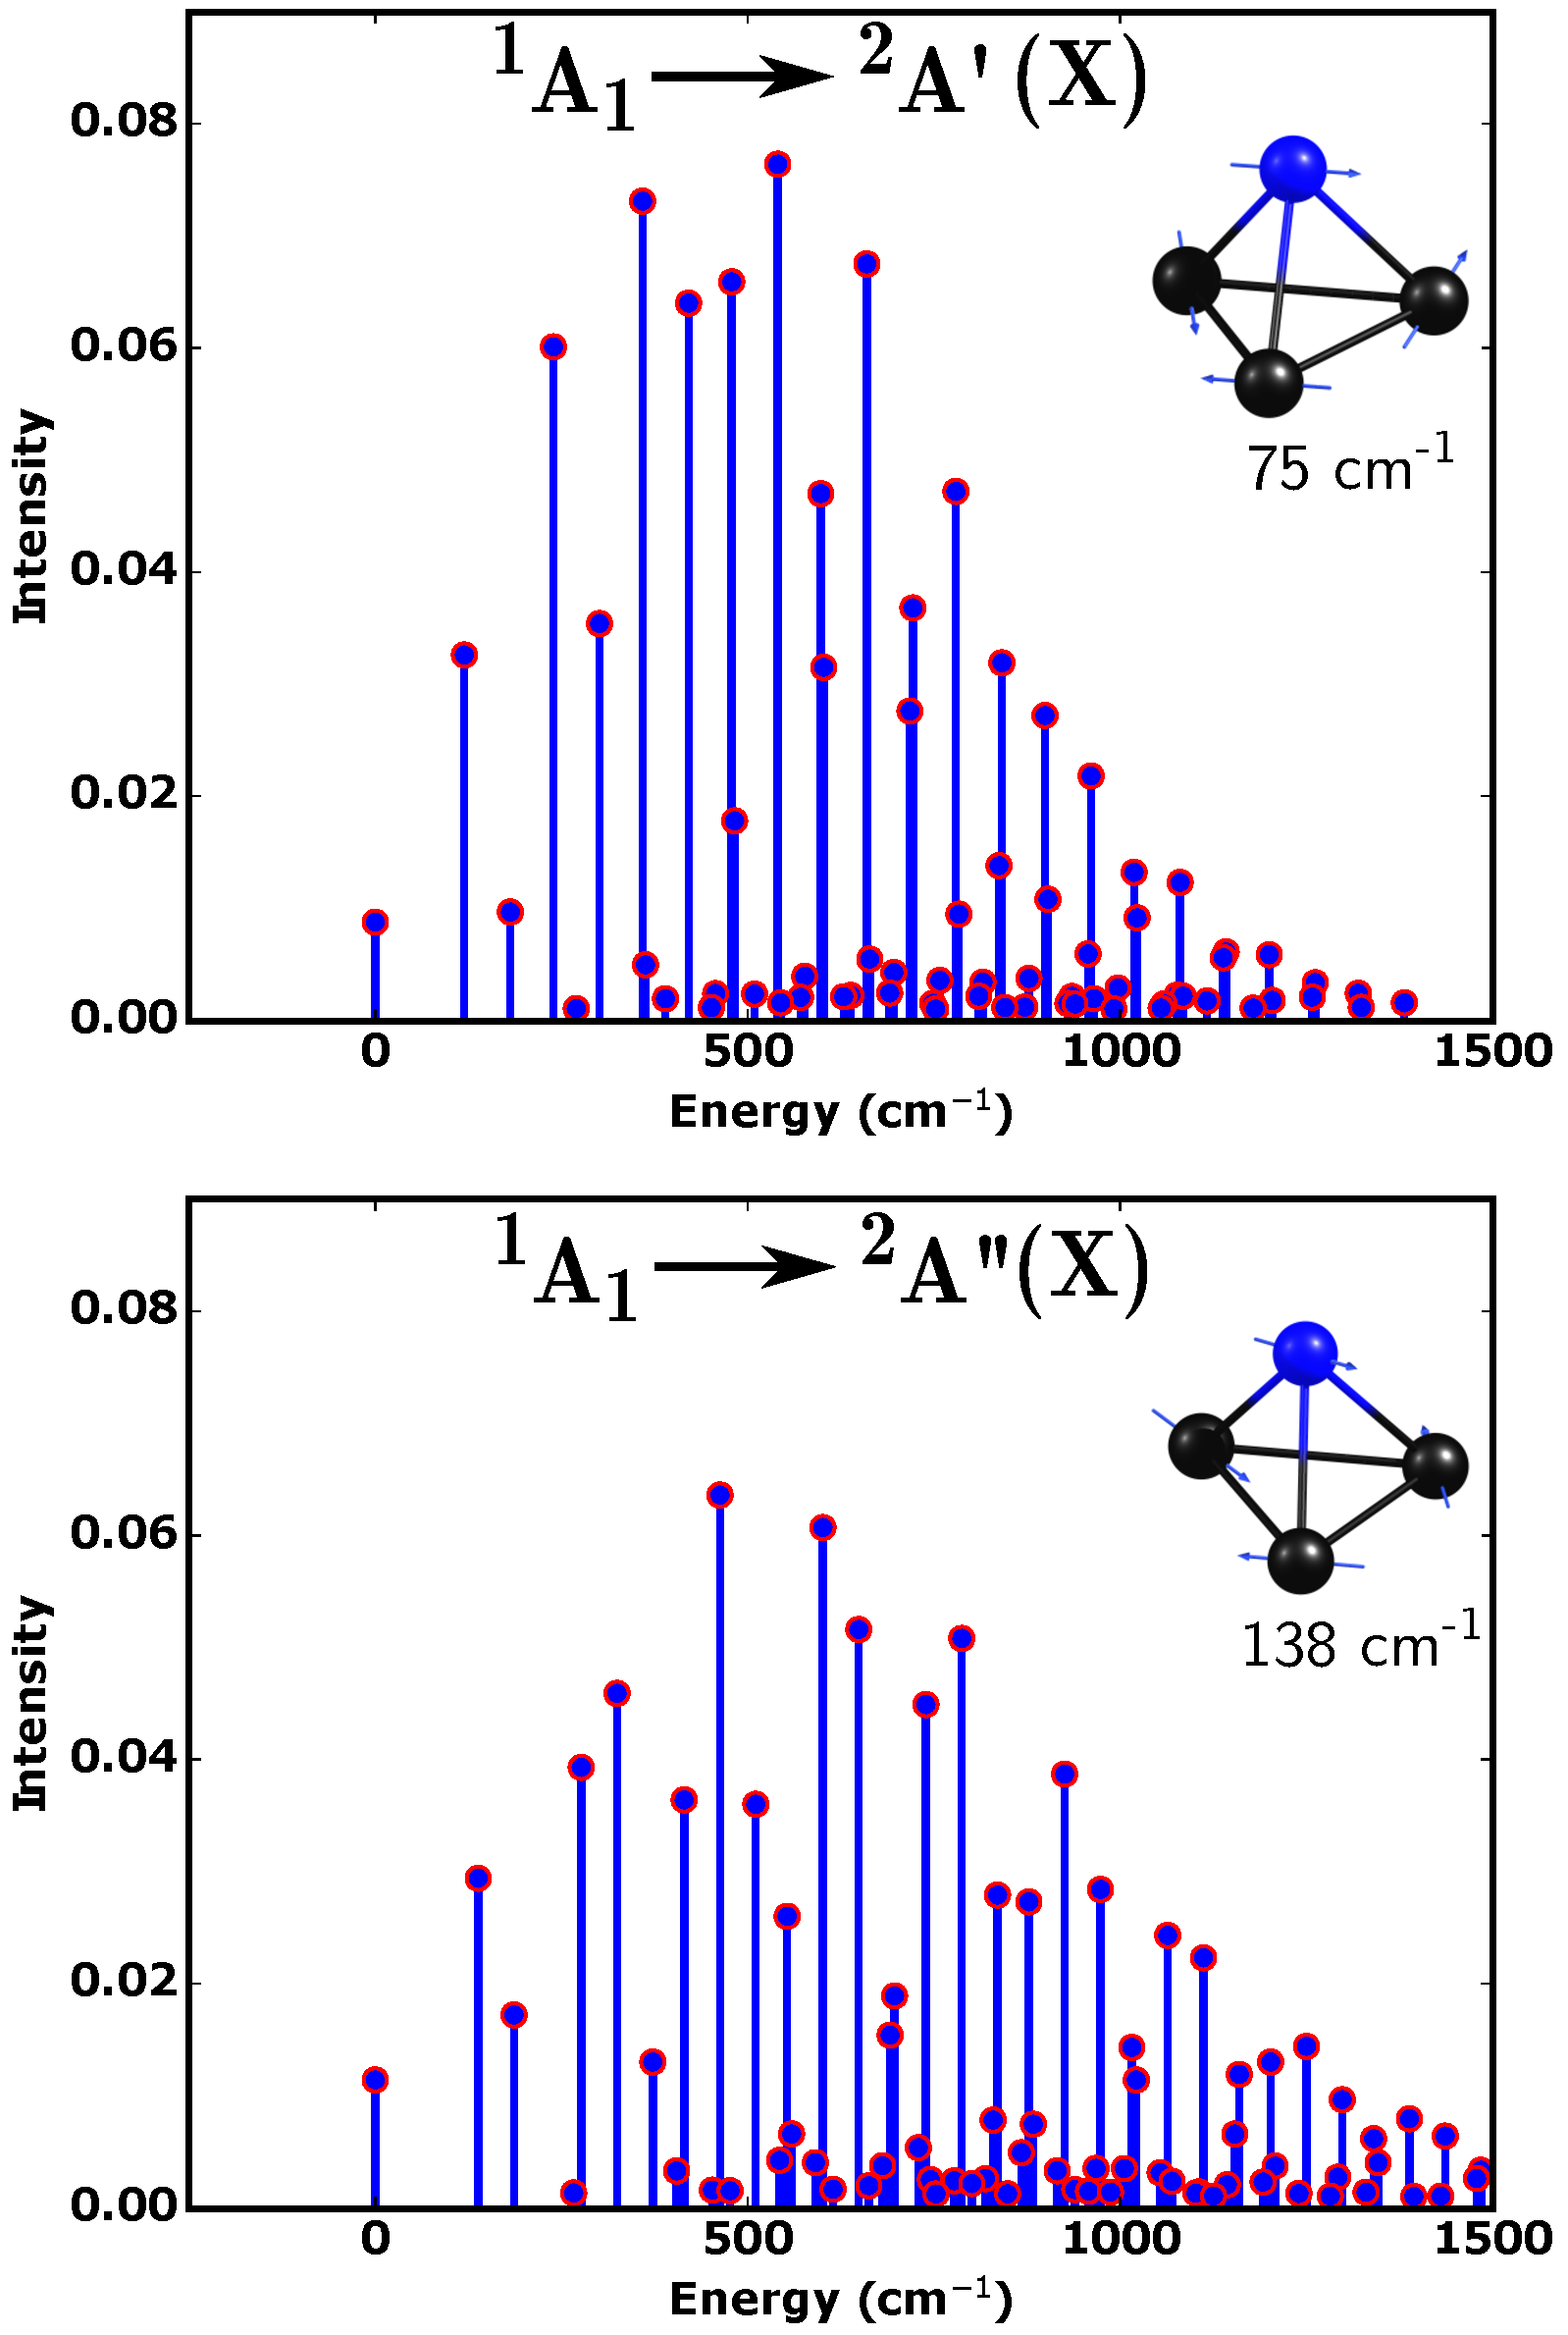
\includegraphics[width=0.5\textwidth]{FC}
    \caption{Franck–Condon factor simulations of two transitions underlying the \acrshort{pe} band X.}
    \label{fig5:FC}
\end{figure} 



\section{Concluding Remarks}



Several geometrical and electronic structures of the tetratomic cluster \ch{VGe3^{-/0}} were investigated using both single-reference and multireference quantum chemical methods. The tetrahedral shape was found to be the most stable isomer of both anionic and neutral \ch{VGe3^{–/0}}. While the anion exhibits a C$_{3v}$ point group, the neutral cluster has a C$_s$ spatial symmetry, due to the Jahn-Teller effect. This result is completely different from previously reported results that the rhombic isomer is the most stable one. Furthermore, a low-spin state $^1$A$_1$ (C$_{3v}$) is the global ground state of the anionic cluster \ch{VGe3-}. Subjected to a Jahn-Teller distortion in two different directions, both resulting $^2$A' and $^2$A" states are the nearly degenerate and competitive ground state of the neutral \ch{VGe3}.





On the basis of the anionic ground state $^1$A$_1$'s electron configuration, four of the five bands experimentally recorded in the anion photoelectron spectrum of \ch{VGe3-} were energetically and electronically assigned. The first band X is the result of two simultaneous electronic transitions from the anionic ground state. The A band was assigned to two other transitions with higher ionization energy. The bands B and C were ascribed to two energetically deeper transitions. The identity of the last band D cannot be assigned, as larger \acrshort{casscf} wave functions are needed to be constructed, and this is presently out of our computing resources. We believe that electronic transitions forming this band likely start from \acrshort{mo}s with larger contributions from the 4s orbitals of germanium atoms. Multidimensional Franck–Condon factor simulations give rise to additional confirmation of the X band's assignment and provide more details about the progression of this band.





As for an energetically reasonable and computationally less demanding theory to treat doped germanium cluster systems like \ch{VGe3^{-/0}}, the pure density functional BP86 emerges as our suggestion for a reliable method.













%%%%%%%%%%%%%%%%%%%%%%%%%%%%%%%%%%%%%%%%%%%%%%%%%%
% Keep the following \cleardoublepage at the end of this file, 
% otherwise \includeonly includes empty pages.
%\cleardoublepage

\includebibliography
\printbibliography[heading=subbibliography] % print section bibliography

\end{refsection}





